\documentclass[11pt]{article}
\usepackage[margin=0.95in]{geometry}
\usepackage{amsmath,amssymb}
\usepackage{tikz}\usepackage{pgfplots}\pgfplotsset{compat=1.18}
\usepackage{xcolor}
\definecolor{ink}{HTML}{1A1B2E}\definecolor{acc}{HTML}{7C3AED}\definecolor{tea}{HTML}{0E9F9A}\definecolor{amb}{HTML}{D97706}\definecolor{ros}{HTML}{E11D48}
\usepackage[colorlinks=true,linkcolor=acc]{hyperref}
\usepackage{titlesec}\titleformat{\section}{\large\bfseries\color{ink}}{\thesection}{.6em}{}
\usepackage{parskip}
\newcommand{\lead}[1]{{\color{acc}\textbf{#1}}}
\begin{document}
\begin{center}{\LARGE\bfseries\color{ink} Busy Beaver, Analysed}\\[3pt]
{\large\color{acc} How one undecided 6-state machine became a problem in ergodic theory}\\[2pt]
{\small BB(6) research program \quad$\cdot$\quad 2026-09-08}\end{center}
\vspace{4pt}\hrule\vspace{8pt}

\section{The machine that won't sit still}
The Busy Beaver number $\Sigma(6)$ is unknown, blocked by a few \lead{holdout} Turing machines whose halting is equivalent to an open arithmetic conjecture. One holdout, watched on its natural macroscopic rhythm, is governed by an explicit integer map $\mathbf R$ on pairs $(a,b)$: two counters that grow, collide, and \emph{renew}. The machine halts exactly when the orbit enters a small \lead{fatal set} --- when the gap between the counters lands in $\{1,3,5\}$.

Deciding whether \emph{one} given seed halts is Collatz-hard. So we asked the softer question Tao answered for Collatz: does \emph{almost every} seed run forever?

\section{From a machine to a Gauss map}
The first-return map of $\mathbf R$ to a natural section is, in the right coordinate, a \lead{countable full-branch piecewise-M\"obius Markov map} $G$ of the interval --- a cousin of the Gauss map from continued fractions. Its branch boundaries are the exact fractions
\[ \rho_{k+1}=\tfrac{1}{3\rho_k+1},\qquad \rho_k=1,\ \tfrac14,\ \tfrac47,\ \tfrac{7}{19},\dots\ \to\ \tfrac{\sqrt{13}-1}{6}. \]
Each branch expands; the whole map has a spectral gap. The left plot shows the return map $z\mapsto z'$ (the expanding M\"obius branches); the right shows its invariant density --- smooth, bounded, the fingerprint of a well-behaved chaotic map.

\begin{center}
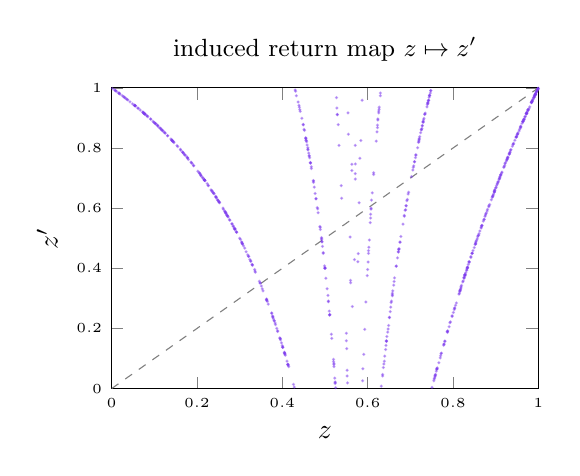
\begin{tikzpicture}\begin{axis}[width=7cm,height=5.4cm,title={\small induced return map $z\mapsto z'$},xlabel={$z$},ylabel={$z'$},xmin=0,xmax=1,ymin=0,ymax=1,tick label style={font=\tiny}]
\addplot[only marks,mark=*,mark size=0.35pt,acc,opacity=0.4] coordinates{(0.056,0.94) (0.384,0.213) (0.061,0.933) (0.378,0.238) (0.235,0.657) (0.676,0.487) (0.64,0.108) (0.683,0.547) (0.798,0.242) (0.141,0.826) (0.56,0.36) (0.734,0.912) (0.985,0.954) (0.819,0.339) (0.054,0.942) (0.533,0.809) (0.972,0.915) (0.387,0.2) (0.951,0.845) (0.876,0.577) (0.238,0.652) (0.492,0.499) (0.077,0.914) (0.171,0.778) (0.871,0.557) (0.5,0.401) (0.9,0.667) (0.213,0.702) (0.038,0.96) (0.521,0.08) (0.6,0.396) (0.906,0.688) (0.815,0.317) (0.72,0.826) (0.651,0.237) (0.77,0.102) (0.552,0.061) (0.69,0.608) (0.972,0.915) (0.055,0.941) (0.972,0.913) (0.563,0.725) (0.706,0.727) (0.973,0.916) (0.302,0.496) (0.976,0.926) (0.002,0.998) (0.336,0.391) (0.658,0.312) (0.431,0.989) (0.854,0.489) (0.932,0.78) (0.731,0.894) (0.378,0.238) (0.999,0.996) (0.964,0.889) (0.131,0.841) (0.923,0.751) (0.999,0.997) (0.966,0.895) (0.407,0.111) (0.686,0.576) (0.726,0.861) (0.818,0.331) (0.539,0.633) (0.912,0.711) (0.538,0.675) (0.73,0.888) (0.868,0.542) (0.624,0.897) (0.994,0.983) (0.139,0.83) (0.244,0.638) (0.952,0.848) (0.245,0.635) (0.939,0.806) (0.309,0.475) (0.21,0.707) (0.346,0.357) (0.672,0.455) (0.927,0.763) (0.658,0.317) (0.218,0.693) (0.167,0.785) (0.293,0.52) (0.235,0.658) (0.555,0.846) (0.868,0.543) (0.266,0.588) (0.632,0.008) (0.69,0.608) (0.178,0.767) (0.217,0.694) (0.859,0.509) (0.401,0.138) (0.233,0.661) (0.389,0.19) (0.772,0.116) (0.383,0.218) (0.696,0.653) (0.531,0.878) (0.03,0.969) (0.326,0.423) (0.031,0.967) (0.909,0.699) (0.788,0.192) (0.721,0.832) (0.838,0.422) (0.912,0.712) (0.414,0.077) (0.306,0.482) (0.857,0.498) (0.609,0.627) (0.89,0.628) (0.658,0.309) (0.884,0.608) (0.928,0.769) (0.413,0.08) (0.092,0.896) (0.984,0.952) (0.948,0.837) (0.24,0.648) (0.405,0.121) (0.656,0.291) (0.958,0.87) (0.305,0.487) (0.521,0.073) (0.833,0.4) (0.741,0.948) (0.735,0.916) (0.654,0.271) (0.838,0.422) (0.214,0.7) (0.853,0.481) (0.218,0.693) (0.289,0.529) (0.553,0.019) (0.992,0.975) (0.496,0.452) (0.289,0.531) (0.744,0.969) (0.726,0.861) (0.692,0.625) (0.627,0.936) (0.834,0.402) (0.577,0.422) (0.493,0.489) (0.655,0.286) (0.674,0.465) (0.804,0.267) (0.516,0.167) (0.816,0.325) (0.908,0.695) (0.473,0.686) (0.793,0.219) (0.893,0.639) (0.131,0.841) (0.853,0.482) (0.289,0.531) (0.727,0.865) (0.608,0.6) (0.271,0.576) (0.622,0.854) (0.663,0.368) (0.91,0.703) (0.589,0.066) (0.463,0.775) (0.988,0.963) (0.801,0.253) (0.832,0.394) (0.824,0.358) (0.012,0.988) (0.914,0.717) (0.076,0.916) (0.396,0.162) (0.282,0.548) (0.52,0.09) (0.505,0.332) (0.073,0.919) (0.177,0.769) (0.858,0.505) (0.143,0.823) (0.287,0.534) (0.817,0.327) (0.569,0.429) (0.466,0.752) (0.083,0.907) (0.529,0.912) (0.401,0.138) (0.743,0.959) (0.307,0.481) (0.758,0.04) (0.976,0.927) (0.083,0.907) (0.603,0.47) (0.591,0.114) (0.728,0.874) (0.863,0.524) (0.945,0.826) (0.623,0.868) (0.028,0.971) (0.741,0.95) (0.034,0.964) (0.324,0.429) (0.187,0.751) (0.601,0.421) (0.272,0.573) (0.123,0.853) (0.934,0.787) (0.406,0.117) (0.873,0.563) (0.244,0.639) (0.951,0.845) (0.606,0.552) (0.265,0.59) (0.897,0.657) (0.644,0.158) (0.103,0.881) (0.46,0.794) (0.689,0.595) (0.826,0.37) (0.219,0.691) (0.63,0.974) (0.959,0.87) (0.686,0.573) (0.076,0.915) (0.967,0.898) (0.025,0.974) (0.73,0.886) (0.806,0.277) (0.167,0.785) (0.482,0.602) (0.834,0.404) (0.653,0.256) (0.206,0.716) (0.483,0.598) (0.648,0.198) (0.74,0.945) (0.381,0.225) (0.46,0.801) (0.693,0.629) (0.985,0.956) (0.881,0.596) (0.986,0.957) (0.845,0.45) (0.814,0.314) (0.893,0.64) (0.466,0.751) (0.009,0.991) (0.449,0.877) (0.161,0.796) (0.124,0.851) (0.455,0.831) (0.563,0.746) (0.969,0.905) (0.892,0.636) (0.118,0.86) (0.511,0.246) (0.484,0.585) (0.441,0.928) (0.473,0.69) (0.02,0.979) (0.178,0.767) (0.823,0.355) (0.406,0.114) (0.007,0.993) (0.582,0.766) (0.695,0.647) (0.83,0.386) (0.604,0.494) (0.92,0.738) (0.55,0.159) (0.639,0.091) (0.248,0.629) (0.321,0.439) (0.524,0.022) (0.189,0.748) (0.828,0.378) (0.528,0.933) (0.415,0.073) (0.389,0.192) (0.996,0.987) (0.993,0.979) (0.63,0.983) (0.252,0.62) (0.102,0.882) (0.829,0.38) (0.676,0.487) (0.433,0.974) (0.608,0.597) (0.473,0.692) (0.866,0.534) (0.524,0.02) (0.703,0.705) (0.614,0.718) (0.261,0.6) (0.466,0.75) (0.99,0.969) (0.855,0.493) (0.075,0.916) (0.933,0.785) (0.511,0.245) (0.413,0.081) (0.428,0.005) (0.578,0.449) (0.659,0.325) (0.771,0.109) (0.713,0.778) (0.4,0.143) (0.673,0.462) (0.489,0.536) (0.751,0.004) (0.647,0.188) (0.794,0.222) (0.941,0.813) (0.724,0.851) (0.759,0.047) (0.209,0.71) (0.607,0.58) (0.381,0.226) (0.249,0.626) (0.949,0.837) (0.661,0.344) (0.853,0.485) (0.964,0.888) (0.721,0.829) (0.268,0.584) (0.554,0.917) (0.898,0.66) (0.282,0.548) (0.552,0.042) (0.873,0.562) (0.268,0.582) (0.861,0.515) (0.319,0.445) (0.398,0.152) (0.969,0.904) (0.145,0.821) (0.926,0.761) (0.607,0.567) (0.455,0.834) (0.626,0.923) (0.584,0.825) (0.649,0.21) (0.335,0.396) (0.798,0.24) (0.828,0.375) (0.71,0.755) (0.262,0.596) (0.952,0.85) (0.779,0.148) (0.009,0.991) (0.964,0.888) (1.0,0.999) (0.998,0.993) (0.218,0.693) (0.18,0.762) (0.852,0.479) (0.984,0.952) (0.571,0.747) (0.894,0.643) (0.826,0.369) (0.627,0.929) (0.525,0.003) (0.895,0.647) (0.787,0.19) (0.055,0.941) (0.921,0.742) (0.363,0.296) (0.492,0.502) (0.834,0.401) (0.273,0.571) (0.239,0.649) (0.761,0.058) (0.192,0.742) (0.588,0.026) (0.226,0.676) (0.929,0.77) (0.719,0.819) (0.897,0.654) (0.808,0.285) (0.043,0.954) (0.452,0.859) (0.146,0.818) (0.71,0.754) (0.468,0.732) (0.411,0.091) (0.72,0.821) (0.529,0.911) (0.394,0.169) (0.842,0.439) (0.293,0.52) (0.353,0.332) (0.667,0.407) (0.638,0.082) (0.468,0.738) (0.364,0.293) (0.678,0.506) (0.276,0.562) (0.571,0.715) (0.395,0.166) (0.745,0.974) (0.901,0.669) (0.842,0.436) (0.993,0.978) (0.073,0.92) (0.745,0.975) (0.781,0.158) (0.993,0.979) (0.494,0.473) (0.992,0.976) (0.174,0.774) (0.626,0.917) (0.928,0.767) (0.762,0.065) (0.85,0.469) (0.479,0.631) (0.728,0.875) (0.107,0.876) (0.155,0.805) (0.144,0.821) (0.932,0.78) (0.475,0.67) (0.925,0.757) (0.707,0.736) (0.904,0.68) (0.623,0.876) (0.5,0.401) (0.91,0.705) (0.828,0.378) (0.091,0.897) (0.166,0.787) (0.312,0.467) (0.803,0.263) (0.52,0.097) (0.063,0.932) (0.1,0.884) (0.62,0.823) (0.169,0.782) (0.523,0.035) (0.758,0.043) (0.973,0.916) (0.348,0.351) (0.099,0.886) (0.017,0.982) (0.405,0.119) (0.99,0.969) (0.44,0.936) (0.955,0.857) (0.787,0.187) (0.115,0.865) (0.984,0.951) (0.993,0.979) (0.643,0.144) (0.268,0.584) (0.515,0.181) (0.3,0.5) (0.984,0.953) (0.018,0.982) (0.477,0.649) (0.932,0.782) (0.993,0.979) (0.834,0.403) (0.635,0.042) (0.192,0.741) (0.524,0.017) (0.108,0.874) (0.237,0.653) (0.878,0.584) (0.972,0.914) (0.456,0.825) (0.108,0.875) (0.763,0.069) (0.252,0.621) (0.571,0.697) (0.171,0.778) (0.277,0.56) (0.832,0.394) (0.207,0.715) (0.912,0.71) (0.253,0.618) (0.377,0.242) (0.991,0.974) (0.734,0.913) (0.708,0.741) (0.363,0.295) (0.078,0.913) (0.897,0.654) (0.458,0.81) (0.266,0.587) (0.564,0.273) (0.375,0.251) (0.103,0.881) (0.927,0.764) (0.499,0.408) (0.306,0.482) (0.305,0.487) (0.976,0.928) (0.645,0.173) (0.763,0.066) (0.446,0.899) (0.365,0.29) (0.964,0.889) (0.074,0.918) (0.755,0.026) (0.919,0.736) (0.828,0.378) (0.978,0.931) (0.902,0.675) (0.599,0.376) (0.922,0.748) (0.602,0.459) (0.508,0.289) (0.602,0.45) (0.351,0.341) (0.559,0.504) (0.33,0.412) (0.457,0.821) (0.904,0.683) (0.153,0.808) (0.395,0.166) (0.756,0.032) (0.787,0.19) (0.999,0.996) (0.492,0.496) (0.249,0.626) (0.285,0.54) (0.46,0.796) (0.202,0.723) (0.875,0.573) (0.508,0.291) (0.496,0.45) (0.521,0.084) (0.224,0.682) (0.779,0.148) (0.527,0.968) (0.739,0.937) (0.049,0.947) (0.053,0.943) (0.98,0.937) (0.56,0.352) (0.111,0.869) (0.186,0.753) (0.33,0.41) (0.747,0.983) (0.363,0.298) (0.126,0.849) (0.426,0.014) (0.866,0.537) (0.551,0.133) (0.27,0.577) (0.5,0.401) (0.644,0.157) (0.489,0.529) (0.942,0.816) (0.941,0.813) (0.757,0.035) (0.962,0.882) (0.355,0.325) (0.826,0.367) (0.036,0.962) (0.791,0.206) (0.413,0.08) (0.141,0.826) (0.375,0.251) (0.479,0.632) (0.017,0.983) (0.205,0.719) (0.845,0.45) (0.085,0.904) (0.329,0.413) (0.43,0.993) (0.321,0.44) (0.886,0.612) (0.73,0.887) (0.326,0.425) (0.067,0.926) (0.742,0.957) (0.097,0.889) (0.12,0.857) (0.67,0.435) (0.367,0.281) (0.762,0.065) (0.958,0.867) (0.898,0.66) (0.315,0.455) (0.935,0.793) (0.507,0.31) (0.745,0.975) (0.5,0.401) (0.748,0.991) (0.462,0.783) (0.593,0.197) (0.743,0.959) (0.596,0.288) (0.949,0.839) (0.449,0.879) (0.437,0.953) (0.55,0.184) (0.079,0.912) (0.767,0.086) (0.759,0.045) (0.251,0.622) (0.456,0.826) (0.637,0.07) (0.227,0.675) (0.804,0.268) (0.58,0.618) (0.348,0.351) (0.571,0.809) (0.997,0.99) (0.288,0.531) (0.51,0.258) (0.587,0.959) (0.285,0.54) (0.673,0.464) (0.778,0.144) (0.973,0.917) (0.292,0.522) (0.672,0.454) (0.217,0.694) (0.999,0.997) (0.995,0.986) (0.991,0.973) (0.722,0.838) (0.667,0.407) (0.993,0.978) (0.88,0.591) (0.624,0.893) (0.845,0.45) (0.455,0.833) (0.442,0.922) (0.405,0.118) (0.915,0.72) (0.877,0.581) (0.379,0.232) (0.141,0.827) (0.741,0.951) (0.635,0.047) (0.054,0.941) (0.897,0.655) (0.688,0.593) (0.836,0.413) (0.956,0.862) (0.644,0.159) (0.816,0.323) (0.867,0.541) (0.114,0.866) (0.909,0.698) (0.986,0.956) (0.502,0.367) (0.906,0.687) (0.976,0.926) (0.884,0.605) (0.337,0.387) (0.463,0.773) (0.989,0.968) (0.82,0.343) (0.611,0.651) (0.838,0.42) (0.209,0.71) (0.713,0.776) (0.078,0.913) (0.712,0.768) (0.996,0.989) (0.773,0.118) (0.987,0.961) (0.966,0.894) (0.439,0.942) (0.464,0.768) (0.717,0.801) (0.948,0.836) (0.642,0.13) (0.488,0.539) (0.959,0.873) (0.614,0.712) (0.732,0.899) (0.662,0.356) (0.966,0.894) (0.493,0.488) (0.819,0.335) (0.86,0.51) (0.217,0.695) (0.245,0.636) (0.651,0.236) (0.271,0.575) (0.162,0.793) (0.142,0.824) (0.511,0.245) (0.401,0.137) (0.847,0.459) (0.974,0.921) (0.119,0.859) (0.817,0.328) (0.936,0.795) (0.748,0.991) (0.451,0.862) (0.781,0.157) (0.828,0.378) (0.116,0.862)};
\addplot[gray,dashed] coordinates{(0,0)(1,1)};\end{axis}\end{tikzpicture}\hfill
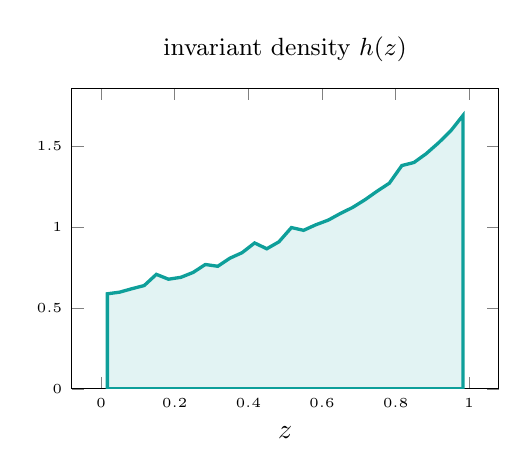
\begin{tikzpicture}\begin{axis}[width=7cm,height=5.4cm,title={\small invariant density $h(z)$},xlabel={$z$},ymin=0,tick label style={font=\tiny}]
\addplot[tea,very thick,fill=tea!12] coordinates{(0.017,0.587) (0.05,0.597) (0.083,0.618) (0.117,0.638) (0.15,0.707) (0.183,0.677) (0.217,0.689) (0.25,0.719) (0.283,0.768) (0.317,0.757) (0.35,0.807) (0.383,0.841) (0.417,0.901) (0.45,0.865) (0.483,0.908) (0.517,0.996) (0.55,0.979) (0.583,1.013) (0.617,1.042) (0.65,1.083) (0.683,1.12) (0.717,1.168) (0.75,1.221) (0.783,1.27) (0.817,1.379) (0.85,1.398) (0.883,1.452) (0.917,1.52) (0.95,1.594) (0.983,1.688)}\closedcycle;\end{axis}\end{tikzpicture}
\end{center}

\section{Two theorems, one proved}
\lead{Measure form (proved).} Lebesgue-almost every real seed never halts. This is a complete theorem: the Gauss-type map has a unique smooth invariant measure with exponential mixing (Rychlik), the size $a+b$ strictly increases every step, and the halting hazard at scale $S$ is $\le 6h(0)/S$, geometrically summable.

\lead{Density form (conditional).} The natural density of halting \emph{integer} seeds is zero. Directly confirmed by counting --- the halting fraction falls like $C/N$:

\begin{center}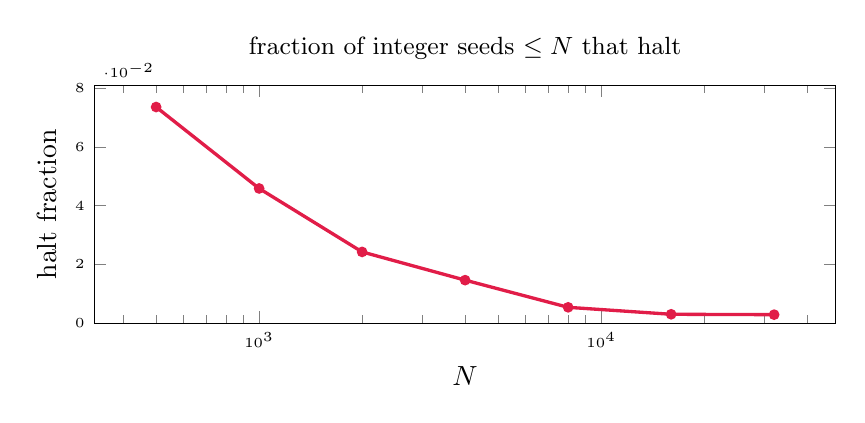
\begin{tikzpicture}\begin{semilogxaxis}[width=11cm,height=4.6cm,title={\small fraction of integer seeds $\le N$ that halt},xlabel={$N$},ylabel={halt fraction},tick label style={font=\tiny},ymin=0]
\addplot[ros,very thick,mark=*,mark size=1.3pt] coordinates{(500,0.07362) (1000,0.04587) (2000,0.02425) (4000,0.01463) (8000,0.00537) (16000,0.003) (32000,0.00287)};\end{semilogxaxis}\end{tikzpicture}\end{center}

But turning that count into a theorem needs the integer orbits to \emph{equidistribute} as well as the measure does --- and that is where harmonic analysis enters. (Companion note: \emph{The Twisted Transfer Operator}.)

\vspace{4pt}\hrule\vspace{4pt}\noindent{\small\color{gray} Every figure is computed from the exact machine. The measure theorem is complete and axiom-checked in Lean at the closure level; the integer-density statement is reduced to a single, precisely stated analytic lemma and remains conditional. No specific seed is decided.}
\end{document}